\documentclass[transmag]{IEEEtran}
\usepackage{latexsym}
\usepackage{graphicx}
\usepackage{amsfonts,amssymb,amsmath}
\usepackage{hyperref}
\usepackage{fancyvrb}
\usepackage{float}
\usepackage{stfloats}
\def\BibTeX{{\rm B\kern-.05em{\sc i\kern-.025em b}\kern-.08em T\kern-.1667em\lower.7ex\hbox{E}\kern-.125emX}}

\begin{document}

\title{Classification of Handwritten Digits using Convolutional Neural Networks
in Tensorflow 2.0}

\author{Charlie Wilkin
\thanks{Submitted December 1st, 2019. This work was completed as part of a 
final project submission for EE456, Intro to Neural Networks.}}

\IEEEtitleabstractindextext{\begin{abstract}
Objective:
Computer vision is a rapidly developing field with a significant
dependence on hardware acceleration and parallel processing. While massively
parallel hardware has existed in some capacity for decades, powerful libraries
enabling its use by untrained indeviduals are a relatively new phenomen. The
launch of Tensorflow 1.0 by Google in 2017 (and more recently, Tensorflow 2.0)
pushed AI-oriented hardware acceleration closer to the mainstream. In this 
project, the beginner-friendly interface of Tensorflow is demonstrated by 
achieving greater than 99\% accuracy on the popular MNIST dataset using fewer
than 50 lines of Python code on consumer hardware.
\end{abstract}

\begin{IEEEkeywords}
Neural Networks, Computer Vision, Parallel Processing, Convolutional Neural Networks
\end{IEEEkeywords}}

\maketitle

\section{Introduction}

\IEEEPARstart{T}{his} project demonstrates one method of achieving greater than
99\% accuracy on the MNIST dataset of handwritten digits. While this
performance is far from state of the art, the implementation is easy to
understand and trains quickly on mid-range consumer hardware. The procedure 
outlined in Section II will assume some rudamentary experience with the
Python programming language, a working install of Tensorflow 2.0 on
a Debian-based system such as Ubuntu, and a compatible Nvidia Graphics
Processing Unit. 

If you do not currently have Tensorflow 2.0 installed with GPU support, you
can follow the directions provided by Google at 
\href{https://www.tensorflow.org/install/gpu}{www.tensorflow.org/install/pip}.
The same webpage outlines the installation of necessary dependencies including
Nvidia drivers, the CUDA toolkit, and the cuDNN software development kit. 
Implementation details regarding the operation of layers within the proposed
model and preparation of the dataset are explained thorougly in Section II. The
full source code for this project is available at 
\href{https://www.github.com/busyboredom/MNISTpaper}
{www.github.com/busyboredom/MNISTpaper}.

\section{Operation and Implementation}

\subsection{Preparing the Dataset}

The MNIST (Modified National Institute of Standards and Technology) dataset
is a collection of 70,000 handwritten digits prepared in 1999 by researchers at
Courant Institute and Google Labs \cite{ref1}. Each image in the MNIST dataset
contains 28x28 grayscale pixels representing a number from 0-9. The images are
centered on the digit and size-normalized, with one-hot encoded labels. Fig. 1
shows one image from the MNIST dataset.

\begin{figure}[H]
  \centerline{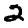
\includegraphics[width=1.5in]{fig1}}
  \caption{A handwritten digit drom the MNIST dataset, consisting of 28x28
  grayscale pixels.\label{fig1}}
\end{figure}

The MNIST dataset is included in Tensorflow, and can be loaded easily by first
importing Tenslorflow and then storing the dataset in a variable.

\begin{figure}[H]
\begin{Verbatim}[samepage=true]
from __future__ import absolute_import, \
                       division, \
                       print_function, \
                       unicode_literals \

import tensorflow as tf

mnist = tf.keras.datasets.mnist
\end{Verbatim}
\end{figure}

The dataset is then divided into seperate training and testing sets.
This allows us to verify the model's performance by testing it on data that it
was not exposed to during training. To accelerate the training process, the 
grayscale pixel values are also normalized to between 0 and 1 by 
dividing each pixel by 255.

\begin{figure}[H]
\begin{Verbatim}
(x_train, y_train), (x_test, y_test) = \
                         mnist.load_data()

x_train, x_test = x_train / 255.0,
                  x_test / 255.0
\end{Verbatim}
\end{figure}

\noindent Finally, a color channel dimension is added to the images. This
dimension is blank, and exists to tell Tensorflow that there are no color
channels in these images.

\begin{figure}[H]
\begin{Verbatim}
x_train = x_train[..., tf.newaxis]
x_test = x_test[..., tf.newaxis]
\end{Verbatim}
\end{figure}

\subsection{Defining the Model}

The model is defined sequentially, layer by layer. The first layer consists
a collection of 32 feature detectors, each 3x3 elements, convolved (i.e. 
scanned across) the image \cite{ref2}. The resulting output is a set of 32 
matrixes, each containing 26x26 elements. To compress this output into 
something more manageable, a 2x2 pooling layer is applied to keep only one out 
of every four pixels before feeding the result into a second layer of 64 
convolutions \cite{ref3}.

\begin{figure}[H]
\begin{Verbatim}
model = tf.keras.models.Sequential([

    tf.keras.layers.Conv2D(
            32, \
            (3, 3), \
            activation='relu', \
            input_shape=(28, 28, 1)),

    tf.keras.layers.MaxPooling2D((2, 2)),

    tf.keras.layers.Conv2D(
            64, \
            (3, 3), \
            activation='relu'),
\end{Verbatim}
\end{figure}

The activation function applied at each element of the 3x3 feature detectors
is known as the ReLU function, or Rectified Linear Unit \cite{ref4}. The ReLU activation 
function (shown in Fig. 2) is popular for its simplicity and its 
easily-calculated derivative. The use of a non-linear function is crucial, as
any sum of purely linear functions will necessarily collapse into a single 
linear function itself.

\begin{figure}[H]
  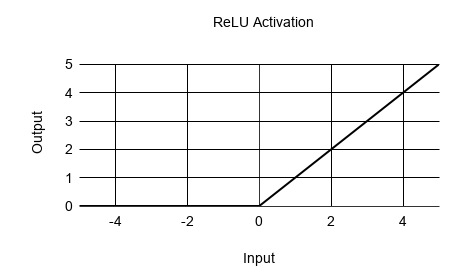
\includegraphics[width=3in]{fig2}
  \caption{The Rectified Linear Unit activation function used throughout 
  this model.\label{fig2}}
\end{figure}

The output of the second convolutional layer is a three dimensional tensor of
shape 11x11x64, and the output of the network as a whole must be a ten 
dimensional output vector. To achieve this, the output of the second 
convolutional layer is first flattened into a single 7744 dimensional vector.
This vector is then fed into a traditional, fully-connected layer of 64 units
with the ReLU activation function.

\begin{figure}[H]
\begin{Verbatim}
    tf.keras.layers.Flatten(),
    tf.keras.layers.Dense(
            64, \
            activation='relu'),
\end{Verbatim}
\end{figure}

Up to this point, a total of 514,496 trainable parameters have been added to
the model. Bearing in mind that the MNIST dataset contains only 70,000 images,
a model of this size risks fitting to random, unintended patterns in the 
training data and failing to generalize to the test data as a result. To
prevent this, the network can be forced to act as a consensus of smaller networks
by randomly eliminating 20\% of the connections in the fully-connected layer
during training \cite{ref5}.

\begin{figure}[H]
\begin{Verbatim}
    tf.keras.layers.Dropout(0.2),
\end{Verbatim}
\end{figure}


The final layer consists of a ten fully-connected units with
the softmax activation function, which compresses the outputs into a values
between 0 and 1 while constraining them such that they add to 1. This causes
the output vector to resemble a probability distribution, where the largest
value represents the predicted digit. 

\begin{figure}[H]
\begin{Verbatim}
    tf.keras.layers.Dense(
            10, \
            activation='softmax')
])
\end{Verbatim}
\end{figure}

\noindent A summary of the complete model, generated using Tensorflow's
\verb model.summary() method, appears in Table I. 

\begin{table}[H]
  \caption{Summary of model, as presented by Tensorflow\label{table1}}
  \centering
  \begin{BVerbatim}
___________________________________________________
Layer (type)       Output Shape            Param #
===================================================
conv2d          (None, 26, 26, 32)        320
___________________________________________________
max_pooling2d   (None, 13, 13, 32)        0
___________________________________________________
conv2d_1        (None, 11, 11, 64)        18496
___________________________________________________
flatten         (None, 7744)              0
___________________________________________________
dense           (None, 64)                495680
___________________________________________________
dropout         (None, 64)                0
___________________________________________________
dense_1         (None, 10)                650
===================================================
Total params: 515,146
Trainable params: 515,146
Non-trainable params: 0
___________________________________________________
  \end{BVerbatim}
\end{table}

\subsection{Training and Evaluating the Model}

Tensorflow provides a number of training algorithms compatible with both
convolutional and fully-connected layers. One such algorithm is a variation of
packpropogation (and by extension, gradient descent) known as Adaptive Moment
Estimation, or Adam \cite{ref6}. Adam adjusts its learning rate automatically
based on the gradients of the weights with respect to the loss function, 
as well as the second moments of those gradients. The model presented in this
project was trained using Adam with an error function equal to the sparse
categorical cross-entropy between the output vector and the one-hot encoded
label.

\begin{figure}[H]
\begin{Verbatim}
model.compile(
    optimizer='adam', \
    loss= \
      'sparse_categorical_crossentropy', \
    metrics=['accuracy'])

\end{Verbatim}
\end{figure}

The model was fit to the training dataset five times before being evaluated on
the test set. The test accuracy, as well as the accuracy after each epoch,
is presented in Section III.

\begin{figure}[H]
\begin{Verbatim}
model.fit(x_train, y_train, epochs=5)

model.evaluate(x_test,  y_test, verbose=2)
\end{Verbatim}
\end{figure}

\section{Results and Conclusion}
 
The model described in Section II was trained on an Nvidia GTX 1060 6GB for 
five epochs before evaluation on the MNIST test dataset. Training lasted 15 
seconds per epoch, for a total of 1.25 minutes. The full test set of 10,000 
images was evaluated by the model in less than one second with greater 99.2\% 
accuracy, misclassifying fewer than 80 images. Table II shows the accuracy and 
loss after each epoch, as well as the final accuracy as presented by Tensorflow 
during training.
 
While the model will not not reliably achieve exactly 99.2\% accuracy without
setting the seed of the random number generator used by Tensorflow, it will
consistently exceed 99\% accuracy after 5 epochs of training regardless of
seed. For the sake of repeatability, a pre-trained model is available at 
\href{https://www.github.com/busyboredom/MNISTpaper}
{www.github.com/busyboredom/MNISTpaper}.

\begin{table*}
  \caption{Accuracy during training and testing, as presented by Tensorflow.
  \label{table2}}
  \centering
  \begin{verbatim}
60000/60000 [==============================] - 15s 243us/sample - loss: 0.1559 - accuracy: 0.9524
Epoch 2/5
60000/60000 [==============================] - 15s 244us/sample - loss: 0.0564 - accuracy: 0.9833
Epoch 3/5
60000/60000 [==============================] - 15s 255us/sample - loss: 0.0393 - accuracy: 0.9871
Epoch 4/5
60000/60000 [==============================] - 15s 248us/sample - loss: 0.0293 - accuracy: 0.9905
Epoch 5/5
60000/60000 [==============================] - 15s 242us/sample - loss: 0.0243 - accuracy: 0.9922
10000/10000 - 1s - loss: 0.0265 - accuracy: 0.9921
  \end{verbatim}
\end{table*}


\pagebreak
\begin{thebibliography}{00}

\bibitem{ref1} Y. LeCun, C. Cortes, C. J. Burges, MNIST Handwritten Digits 
    Database; AT\&T Bell Laboratories, 2010.

\bibitem{ref2} Y. LeCun, B. Boser, J. S. Denker, D. Henderson, R. E. Howard, 
    W. Hubbard, L. D. Jackel, Backpropagation Applied to Handwritten Zip Code 
    Recognition; AT\&T Bell Laboratories, 1989.

\bibitem{ref3} Yamaguchi, Kouichi; Sakamoto, Kenji; Akabane, Toshio; Fujimoto, 
    Yoshiji (November 1990). A Neural Network for Speaker-Independent Isolated 
    Word Recognition. First International Conference on Spoken Language 
    Processing (ICSLP 90). Kobe, Japan.

\bibitem{ref4} Hahnloser, R.; Sarpeshkar, R.; Mahowald, M. A.; Douglas, 
    R. J.; Seung, H. S. (2000). "Digital selection and analogue amplification 
    coexist in a cortex-inspired silicon circuit". Nature. 405: 947–951.


\bibitem{ref5} Hinton, Geoffrey E.; Srivastava, Nitish; Krizhevsky, Alex; 
    Sutskever, Ilya; Salakhutdinov, Ruslan R. (2012). "Improving neural 
    networks by preventing co-adaptation of feature detectors".

\bibitem{ref6} Diederik, Kingma; Ba, Jimmy (2014). "Adam: A method for 
    stochastic optimization".

\end{thebibliography}

\end{document}
